% -----
% COMP 3630 Assignment 02
% Jimmy Lin
% -----
% -
%{{{
\documentclass[11pt,a4paper]{article}
\usepackage{geometry}
\usepackage{amsthm}
\usepackage{amsmath}
\usepackage[colorlinks,
            linkcolor=blue,
            anchorcolor=red,
            citecolor=green
            ]{hyperref}
\usepackage{fancyheadings}
\usepackage{graphicx}
\usepackage{tikz}
\usetikzlibrary{automata,positioning}
\geometry{top=18mm,bottom=18mm,left=20mm,right=20mm}
%}}}
% new command list
%{{{
\newcommand{\AUTHOR}{Jimmy Lin}
\newcommand{\UID}{u5223173}
\newcommand{\UNIVERSITY}{Australian National University}
\newcommand{\COLLEGE}{College of Engineering and Computer Science}
\newcommand{\COURSE}{COMP3630 Theory of Computation}
\newcommand{\LECTURER}{Jinbo Huang}
\newcommand{\LECTURERt}{Dirk Pattinson}
\newcommand{\TASK}{Assignment 02}
\newcommand{\RELEASEDATE}{April. 15 2013}
\newcommand{\DUEDATE}{April. 29 2013}
\newcommand{\TIMECONSUME}{23h}
%}}}
\newcommand{\htab}{\hspace*{0.63cm}}
\newcommand{\dhtab}{\hspace*{1.2cm}}
\newcommand{\ba}{\hspace*{0.2cm} | \hspace*{0.2cm}}
\newcommand{\pg}{\\[0.3cm]}
\newcommand{\lmd}{\underset{lm}{\Longrightarrow}}
\newcommand{\rmd}{\underset{rm}{\Longrightarrow}}
\newcommand{\mlmd}{\overset{*}{\underset{lm}{\Longrightarrow}}}
\newcommand{\mrmd}{\overset{*}{\underset{rm}{\Longrightarrow}}}
\newcommand{\ps}{P_{Stack}}
\newcommand{\pdaid}[2]{(q, #1, #2)}
\newcommand{\idDerive}[1]{\underset{\ps}{\vdash}}
\newcommand{\Y}{Y_{0}}
\newcommand{\LL}{L^{*}}
%\newcommand{\item}[1]{\hspace*{3cm} #1}
% -
\pagestyle{fancyplain}
\lhead{\COURSE}     
\rhead{\TASK}  
\lfoot{\copyright \AUTHOR (\UID)}
\rfoot{\UNIVERSITY}
% - 
\begin{document}
% ---------------------------
%{{{
\begin{titlepage}
    \begin{center}
        \vspace*{0.8cm}
% add uni photo here.
\includegraphics[width=0.2\textwidth]{/Users/JimmyLin/ANU.png}\\[1cm]
\textsc{\LARGE \UNIVERSITY}\\[1.5cm]

% Title
\rule{\linewidth}{0.5mm} \\[0.4cm]
{ \textsc{\Large \COURSE}\\[0.5cm]
 \huge \bfseries \TASK}\\[0.4cm]
 \footnotesize Edited by \LaTeX \\[0.25cm]
 \normalsize{\COLLEGE}
\rule{\linewidth}{0.5mm} \\[1.5cm]

% other information
\begin{center}
\copyright \emph{\large Author} \\
\Large \textbf{\AUTHOR} \\ \UID \vspace*{0.6cm}

\P \emph{ Lecturer} \\
\Large \textbf{\LECTURER} \vspace*{0.6cm}

\P \emph{ Lecturer} \\
\Large \textbf{\LECTURERt} \vspace*{0.6cm}


$\dagger$ \emph{Release Date}  \\
\Large \textbf{\RELEASEDATE} \vspace*{0.6cm} 

$\ddagger$ \emph{Due Date}  \\
\Large \textbf{\DUEDATE} \vspace*{0.6cm}

$\tau$ \emph{Time Spent} \\
\Large \textbf{\TIMECONSUME} \vspace*{0.6cm} 
\end{center}
% foot
\vfill
{\large \today}
\end{center}
\end{titlepage}

% table of content
\begin{center} \tableofcontents \end{center}
 \newpage
%}}}
% --------------------------
% Exercise 1 
 \section{Proof by Induction}
  \htab Consider the CFG $G$ defined by productions:
    $$ S \rightarrow aS \ba Sb \ba a \ba b $$
% 1.1 Prove by induction on the string
%{{{
 \subsection{Prove by induction on the string}
\htab {Prove by induction on the string length that no string in $L(G)$ has ba as a substring.} \pg
\htab In $L(G)$, it is impossible for those strings, whose length is 0 and 1, to have $ba$ as substring, since the length of a string cannot be smaller than its substring. Hence, we just need to make mathematical induction for the string whose length is no less than 2 ($n \geq 2$). \\[0.1cm]
\htab \textbf{Base Case}: for $n = 2$, prove that 
    $$\forall string\ w \in L(G)\ and\ |w| = 2,\ have\ no\ substring\ ba$$ 
\htab \textbf{Proof:}\\
\htab All possible derivations for string of length 2 are as follows,
    \begin{equation}  \label{S1}
        S \Rightarrow aS \Rightarrow aa 
    \end{equation}
    \begin{equation} \label{S2}
        S \Rightarrow aS \Rightarrow ab
    \end{equation}
    \begin{equation} \label{S3}
        S \Rightarrow Sb \Rightarrow ab
    \end{equation}
    \begin{equation} \label{S4}
        S \Rightarrow Sb \Rightarrow bb
    \end{equation}
\htab It can be seen from above derivations that all possible strings of length 2 are,
    $$ aa,\ ab,\ bb $$
\htab Obviously, $ba$ is not included in the possible set of strings of length 2. Therefore, NO strings of length two in language $L(G)$ has substring $ba$. Formally, we have  
    \begin{equation}
         \forall string\ w \in L(G)\ and\ |w| = 2,\ have\ no\ substring\ ba.
    \end{equation}
\htab \textbf{Inductive Cases}: for arbitrary $n\geq 2$ \\
\htab Assume that 
    \begin{equation} \label{1:precondition}
         \forall \ string\ w\in L(G)\ and\ |w| = m,\ have\ no \ substring\ ba
    \end{equation}
\htab Prove that for string of length $m+1$ have the same property. Formally
    \begin{equation} \label{1:postcondition}
         \forall \ string\ w' \in L(G)\ and\ |w'| = m+1,\ have \ no \ substring\ ba
    \end{equation}
\htab \textbf{Proof:}\\
\htab We consider the first-step derivation for string $w'$. There are two possible cases based on the production of grammar $G$.
\begin{align}
    \textbf{First case: } S \Rightarrow aS \Rightarrow aw \htab w' &= aw \\
    \textbf{Second case: } S \Rightarrow Sb \Rightarrow wb \htab w' &= wb
    \end{align}
\htab Based on the inductive hypothesis \eqref{1:precondition}, the string $w$ of length $m$ always has no substring $ba$. We use this property of string $w$ to derive the followings,
        \begin{itemize}
    \item{First Case: We have shown that no substring $ba$ in string $w$ (inductive hypothesis). Besides, whatever the first letter of string $w$ is $a$ or $b$, append one $a$ in head of the string $w$ will not introduce occurence of $ba$. Therefore, in this case, string $w'$ of length $m+1$ has no substring $ba$.}
    \item{Second Case: We have shown that no substring $ba$ in string $w$ (inductive hypothesis). Besides, whatever the last letter of string $w$ is $a$ or $b$, append one $b$ in tail of the string $w$ will not introduce occurence of $ba$. Therefore, in this case, string $w'$ of length $m+1$ has no substring $ba$.}
        \end{itemize}
\htab In summary, we have proven that there is no substring $ba$ in any string of length $m+1$ given no substring $ba$ in any string of length $m$. That is, the inductive cases hold. According to the principle of mathematical induction, it is concluded that
\begin{align}
    \forall string\ w \in L(G),\ |w| \geq 2,\ w\ have\ no\ substring\ ba
\end{align}
\htab Since the string of length 0 or 1 in the language of grammar $G$ is impossible to have substring $ba$, as we discussed in the very beginning, it can be concluded that
\begin{align}
    \text{NO string in $L(G)$ has $ba$ as a substring.}
    \end{align}
%}}}
\newpage
% 1.2 Describe $L(G)$ informally
%{{{
\newcommand{\Lone}{L_{1}}
\newcommand{\Ltwo}{L_{2}}
\newcommand{\Ltwob}{\overline{L_{2}} }
\newcommand{\ws}{w^{*}}
\newcommand{\wsp}{w^{*'}}
\subsection{Describe $L(G)$ informally}
\htab {Describe $L(G)$ informally. Justify your answer using part (1).} \pg
\htab To get the informal description, we observe some patterns from those production rules that contain variable in the body. 
\begin{itemize} \renewcommand{\labelitemi}{$\diamond$}
    \item{ terminal $a$ always occur before the variable $S$}. 
    \item{ $b$ always occurs after variable $S$}. 
    \item{ variable $S$ by itself can be instantiated to both terminal $a$ and $b$}.
\end{itemize}
\htab Based on the observation above, the informal description of $L(G)$ is as follows,
\begin{equation}
    L(G) = \{ \text{all occurrences of $a$ come before any occurrence of $b$} \}
    \end{equation}
\htab Then justify my answer. \pg
\htab Let $L_{1}$ to be set of strings in which all occurrences of $a$ come before any occurrence of $b$,
and let $L_{2}$ to be the set of strings that contains $ba$ as a substring.
Now, our ultimate objective is to prove that $L(G) = L_{1}$. \\
\htab But first we should prove another lemma, that is
\begin{align}
    \Ltwob = \Lone \label{1:lemma}
    \end{align}
\htab To prove this lemma, we should prove both of followings, 
\begin{align}
    \Ltwob \subseteq \Lone  \label{1:lemmaa}\\
    \Lone \subseteq \Ltwob  \label{1:lemmab}
    \end{align}
\htab First things first, we prove \eqref{1:lemmaa}, that is to prove 
\begin{align}
    \forall w \in \Ltwob,\ w \in \Lone
    \end{align}
\htab \textbf{Prove it by contradition}. Assume that there exists $\ws \in \Ltwob,\ \ws \not \in \Lone$.
Since $\ws$ is not in $\Lone$, there exists some $b$ before $a$ in the string $\ws$. Thus, we can
write $\ws = ZbXaY$, where $Z,X,Y$ are arbitrary strings. Then we use induction on the length of 
$X$ to prove $\ws$ must have substring $ba$, that is $\ws \not \in \Ltwob$. \\
\htab \textbf{Base Case}, when $|X| = 0$, we have $\ws = ZbaY$, which apparently has substring $ba$. \\
\htab \textbf{Inductive Cases}, assume that for $|q| = n$, $\ws = ZbqaY$ has substring $ba$, prove that 
for $|q'| = n + 1$, $\wsp = Zbq'aY$ has substring $ba$. Because the $|q'| = |q| + 1$, we have two possibilities
for the form of $q'$. They are $q' = qa$ and $q' = qb$. 
\begin{itemize}
    \item{In case of $q' = qa$, $\wsp = Zbq'aY = ZbqaaY$ and because
        we have shown in the inductive hypothesis that $ZbqaY$ has substring $ba$, obviously $\wsp = ZbqaaY$ must have substring $ba$.}
    \item{In the case of $q' = qb$, we have $\wsp = Zbq'aY = ZbqbaY$, which apparently has substring $ba$. } 
\end{itemize}
\htab As shown above, we prove that $\ws$ must have substring $ba$, which contradicts to our assumption that 
$\ws \in \Ltwob$. Therefore, we should negate the assumption and conclude that
    $\forall w \in \Ltwob,\ w \in \Lone$. Hence, we have $\Ltwob \subseteq \Lone$.\pg
\htab Then, we turn to prove $\Lone \subseteq \Ltwob$ \eqref{1:lemmab}, that is to prove
\begin{align}
    \forall w \in \Lone,\ w \in \Ltwob \label{1:foralllLemmaa}
\end{align}
\htab We can \textbf{prove it by contradiction}. Assume there exists $\ws \in \Lone, \ws \not \in \Ltwob \ holds$.
since $\ws \not \in \Ltwob$, $\ws$ have substring $ba$, which make $\ws$ not in $\Lone$ because we 
have the definition of $\Lone$ is that all occurrence $a$ comes before $b$. Therefore, we prove 
\eqref{1:foralllLemmaa} by negating the assumption. \\
\htab Until now, we proved the \eqref{1:lemmaa} and \eqref{1:lemmab}, 
so we achieved the proof of $\Ltwob = \Lone$. \pg
\htab Now let us start to prove the ultimate objective, $L(G) = L_{1}$. We should prove both of followings, 
\begin{align}
    L(G) \subseteq L_{1} \\
    L_{1} \subseteq L(G) 
    \end{align}
\htab \textbf{Proof for $L(G) \subseteq \Lone$}:\\
\htab The result of part (1) demonstrates that 
\begin{align}
    L(G) \subseteq \Ltwob
    \end{align}
\htab Since we have proven the lemma \eqref{1:lemma} $\Ltwob = \Lone$, 
\begin{align}
    L(G) \subseteq \Lone
    \end{align}
\htab \textbf{Proof for $\Lone \subseteq L(G)$}: \\
\htab To prove $\Lone \subseteq L(G)$, we need to show that for any string $w \in \Lone$,
it holds that $ w \in L(G)$. We prove this by induction on the length of string $w$. \\
\htab \textbf{Base Case}: when $|w| = 1$, it is true without any doubt because $a$ and $b$ are
both in $\Lone$ and $L(G)$.
\htab \textbf{Inductive Case}: Postulate the claim that if $w \in \Lone$, then $w \in L(G)$ 
holds for $|w| = n$, show that this claim still holds for $|w'| = |w| + 1 = n+1$. \\
\htab Since $w' \in \Lone$, we have two possibilities for the form of $w'$ whose length is $n+1$, that is,
    \begin{align}
        \text{$a^{i}b^{n+1-i}\ (0 \leq i \leq n+1)$ or $b^{n+1}$}. 
    \end{align}
\begin{itemize}
\item{In the case of $w' = a^{i}b^{n+1-i} = a a^{i-1}b^{n+1-i}$, since $w = a^{i-1}b^{n+1-i}$ is 
        of length $n$ and belongs to $L_{1}$, $w \in L(G)$ according to inductive hypothesis.
        Hence, $w'$ can be derived by $S \Rightarrow aS \Rightarrow  a a^{i-1}b^{n+1-i} $.}
\item{The other case is that $w' = b^{n+1}$, and similarly we can derive the string $w'$ by
    $S \Rightarrow bS \Rightarrow b b^{n}$.}
\end{itemize}
\htab It can be concluded by those two cases above, if $w' \in \Lone$, $w'$ can always
be derived by grammar $G$ given $w = |w'| - 1$ belongs to $\Lone$ and $L(G)$. \\
\htab Therefore, we prove that if $w \in \Lone$, then $w \in L(G)$, that is to say, $\Lone \subseteq L(G)$. \pg
\htab All in all, we fulfill the proof for $L(G) \subseteq L_{1}$ and $L_{1} \subseteq L(G)$. Hence,
$L(G) = L_{1}$ holds. That is, 
\begin{align}
    L(G) = L_{1} = \{ \text{all occurrences of $a$ come before any occurrence of $b$} \}
    \end{align}
 \newpage
%}}}
% Exercise 2 
 \section{Unambiguous Grammars}
\htab The following grammar generates prefix expressions with operands $x$ and $y$ and binary operators $+,-,*$,
    $$ E \rightarrow +EE \ba \times EE \ba - EE \ba x \ba y $$
% 2.1 Give leftmost and rightmost derivations, and a parse tree
%{{{
\subsection{Give leftmost and rightmost derivations, and a parse tree}
\htab Give leftmost and rightmost derivations, and a parse tree for the string +*-xyxy. \pg
\htab First left-most derivation for string +*-xyxy,
    \begin{align}
        E & \lmd +EE &&\mbox{by $E \rightarrow +EE$} \\
          & \lmd +\times EEE &&\mbox{by $E \rightarrow \times EE$}\\
              & \lmd +\times - EEEE &&\mbox{by $E \rightarrow -EE$}\\ 
              & \lmd +\times -xEEE &&\mbox{by $E \rightarrow x$}\\
              & \lmd +\times -xyEE &&\mbox{by $E \rightarrow y$}\\
              & \lmd +\times -xyxE  &&\mbox{by $E \rightarrow x$}\\
              & \lmd +\times -xyxy &&\mbox{by $E \rightarrow y$}
    \end{align}
\htab Then right-most derivation for string +*-xyxy,
    \begin{align}
            E & \rmd +EE &&\mbox{by $E \rightarrow +EE$}\\
              & \rmd +Ey &&\mbox{by $E \rightarrow y$}\\
              & \rmd +\times EEy &&\mbox{by $E \rightarrow \times EE$}\\ 
              & \rmd +\times Exy &&\mbox{by $E \rightarrow x$}\\
              & \rmd +\times -EExy &&\mbox{by $E \rightarrow -EE$}\\
              & \rmd +\times -Eyxy  &&\mbox{by $E \rightarrow y$}\\
              & \rmd +\times -xyxy &&\mbox{by $E \rightarrow x$}
    \end{align}
\htab Finally, the parse tree (yield) for string +*-xyxy,
    \begin{center}
        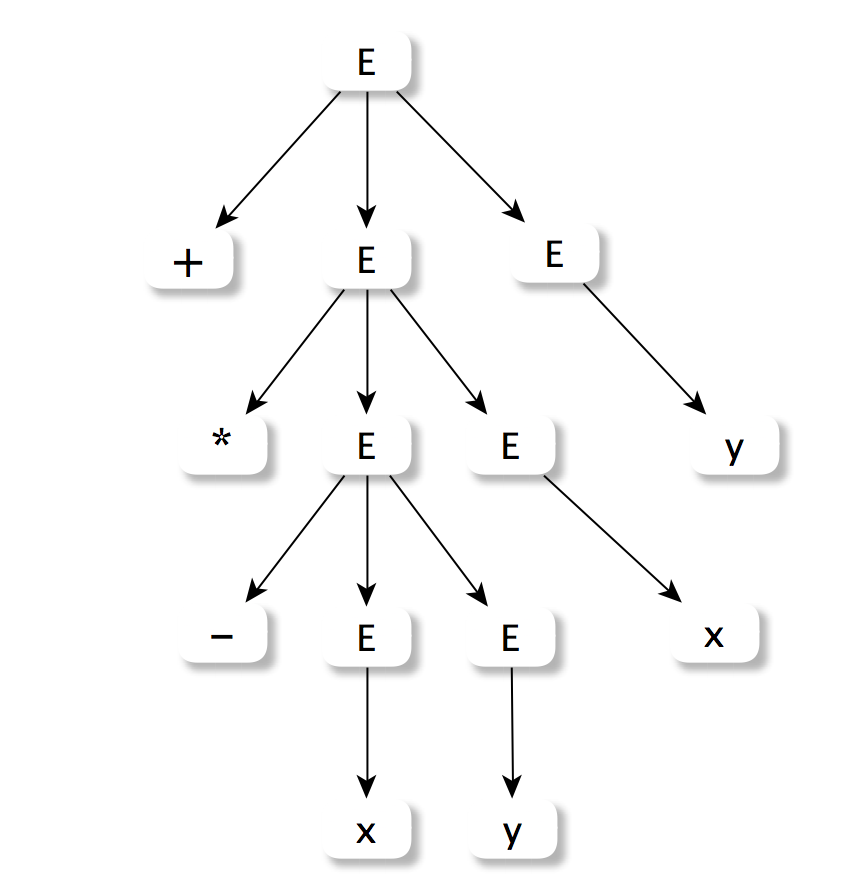
\includegraphics[width=3in,height=3in]{./graphs/parseTree.png}\\
        \footnotesize Fig. Parse Tree for word +*-xyxy
    \end{center}
\newpage
%}}}
% 2.2 Prove unambiguity of given grammar 
%{{{
\subsection{Prove unambiguity of given grammar}
\htab Prove that this grammar is unambiguous. \pg
\htab To prove the unambiguity of the grammar, we need to prove that the leftmost derivation for 
all strings in that language are unique. That is,
\begin{align} 
    \forall \text{string } w \in L(G),\ E \mlmd w \text{ is unique.} \label{2:lemma}
    \end{align}
\htab \textbf{Proof}: Mathematical induction implemented on the nubmer of steps of "expanded derivation",
under which there is one variable $E$ instantiated to $+EE \ba \times EE \ba -EE$. (Note that we 
just call such derivation as "expanded derivation" for that only "expanded derivation" will enlarge
the length of string. And by contrast, $E \rightarrow x \ba y$ is not "expanded derivation".) \\
\htab Notational definition: $E_{k}$ represents one variable $E$ to be instantiated to a string 
with $k$ step expanded derivation.  \pg
\htab \textbf{Base Case}: For those strings with no expanded derivation in the language of 
grammar E, it is evident that they are unique in leftmost derivation. 
    \begin{align}
        E_{0} \mlmd x \\
        E_{0} \mlmd y 
        \end{align}
\htab \textbf{Inductive Cases}: \\
\htab Assume that the 
\begin{align} 
    \text{$\forall$ string $r$, obtained by $k$ step expanded derivation, $E_{k} \mlmd r$ is unique.}
    \end{align}
\htab Prove that 
\begin{align}
    \text{$\forall$ string $r'$, obtained by $k+1$ step expanded derivation, $E_{k+1} \mlmd r'$ is unique.}
    \end{align}
\htab \textbf{Proof}:\\
\htab Generally, we consider first step of leftmost derivation for variable $E$ with $k+1$ expanded derivation. There are three possibibilities as follows,
\begin{align} 
    E_{k+1} \lmd + E_{i} E_{j} \\
    E_{k+1} \lmd \times E_{i} E_{j} \\
    E_{k+1} \lmd - E_{i} E_{j} 
    \end{align}
\htab where $i$ is the number of expanded derivation to be instantiated in the first variable, 
while $j$ is that of second variable $E$. $i+j=k$, which means there are 
still $k$ step expanded derivation in total remained for the 
the first $E$ and second $E$ in right-hand side of above derivation. \\
\htab Written in a compact form as follows, 
\begin{align}
    E_{k+1} \lmd (+\ | \times | -) E_{i} E_{j} \label{2:firstEXP}
    \end{align}
\htab Since $i+j=k$, $i \geq 0$ and $j \geq 0$, it can be obtained that
\begin{align} \label{2:unequal}
    \text{$i \leq k$ and $j \leq k$}
    \end{align}
\htab Now we need to use the following lemma, which obviously holds. 
(The proof for this lemma is provided after the solution for this question.
We just uses it first without interrupting this proof.) \\
\htab \textbf{Lemma}: if leftmost derivation for $E_{x}$ is unique,
the leftmost derivation for $E_{y}\ (y < x)$ must be unique. \\ 
\htab According to the introduced lemma, since $i \leq k$ and $j \leq k$ (see \eqref{2:unequal})
 and $E_{k}$ is unique (inductive hypothesis), it is concluded that 
\begin{align}
    \text{$E_{i}$ and $E_{j}$ are both unique in its leftmost derivation.}
    \end{align}
\htab Therefore, leftmost derivation for $E_{k+1}$ is unique because 
all terminals and variables in its first expanded derivation \eqref{2:firstEXP} is unique. \\
\htab Hence, by principle of mathematical induction, it is concluded that all strings 
that are derived in by grammar $G$ in leftmost derivation is unique, which is sufficient to 
induce the unambiguity of the grammar $G$ by definition of unambiguity.\pg
\hrule \vspace*{0.2cm}
Now we prove the lemma introduced in the above proof. \\
\htab \textbf{Lemma}: if leftmost derivation for $E_{x}$ is unique,
the leftmost derivation for $E_{y},\ (y < x)$ must be unique. \\
\htab We prove this by contradiction. \\
\htab It is known that leftmost derivation for $E_{x}$ is unique, and we assume that 
leftmost derivation $E_{y}(y < x)$ is not unique. \\
\htab The $E_{x}$ can be represented as,
\begin{align}
    E_{x} \lmd (+|\times | -)E_{y} E_{x-y-1}
    \end{align}
\htab Since the $E_{y}(y<x)$ is not unique in its leftmost derivation, \textbf{$E_{x}$ must not be unique}. 
This is because $E_{x}$ has one component $E_{y}$, which is not unique.\\
\htab Therefore, we find a contradiction that $E_{x}$ cannot be both unique and not unique,
for which we should negate the assumption that $E_{y}(y<x)$ is not unique. That is to say,
\begin{align}
    \text{ if $E_{x}$ is unique, then $E_{y}(y < x)$ must be unique.}
    \end{align}
\newpage
%}}}
% Exercise 3
\section{Acceptance by Final State vs. Empty Stack}
\htab Consider the PDA $P = (\{p, q\}, \{ 0, 1\}, \{Z_{0}, X\}, \delta, Z_{0}, q,\{p\})$, 
whose transition function is,
    \begin{align}
        \delta(q, 0, Z_{0}) &= \{ (q, XZ_{0})\} \\
        \delta(q, 0, X) &= \{ (q, XX)\} \\
        \delta(q, 1, X) &= \{ (q, X) \} \\
        \delta(q, \epsilon, X) &= \{ (p, \epsilon)\} \\
        \delta(p, \epsilon, X) &= \{ (p, \epsilon)\} \\
        \delta(p, 1, X) &= \{ (p, XX)\} \\
        \delta(p, 1, Z_{0}) &= \{ (p, \epsilon)\} 
    \end{align}
% 3.1 Convert P to another PDA that accepts by empty stack
%{{{
\subsection{Convert P to another PDA that accepts by empty stack}
\htab Convert P to another PDA $P_{1}$ that accepts by empty stack the same language that $P$ accepts by final state; i.e., $N(P_{1}) = L(P)$. \pg
\htab To establish an equivalent PDA with acceptance by empty stack, we utilize an additional state $s_{0}$ to introduce the initial bottom of statck $Z_{0}$ in the original PDA $P$, and another new state $s_{f}$ to label acceptance.\\
\htab The $P_{1}$ we construct is $(\{s_{0}, s_{f}, p, q\}, \{ 0, 1\}, \{\Y, Z_{0}, X\}, \delta, \Y, s_{0})$, transition functions are as follows,
    \begin{align}
        \delta(q, 0, Z_{0}) &= \{ (q, XZ_{0})\} \\
        \delta(q, 0, X) &= \{ (q, XX)\} \\
        \delta(q, 1, X) &= \{ (q, X) \} \\
        \delta(q, \epsilon, X) &= \{ (p, \epsilon)\} \\
        \delta(p, \epsilon, X) &= \{ (p, \epsilon), (s_{f}, \epsilon)\} \label{PDA:new0}\\
        \delta(p, 1, X) &= \{ (p, XX)\} \\
        \delta(p, 1, Z_{0}) &= \{ (p, \epsilon)\} \\
        \delta(s_{0}, \epsilon, \Y) &= \{ (q, Z_{0}\Y)\} \label{PDA:new1} \\
        \delta(p, \epsilon, Z_{0}) &= \{ (s_{f}, \epsilon)\} \label{PDA:new2} \\
        \delta(p, \epsilon, \Y) &= \{ (s_{f}, \epsilon)\} \label{PDA:new3} \\
        \delta(s_{f}, X, \epsilon) &= \{ (s_{f}, \epsilon)\} \label{PDA:new4} \\
        \delta(s_{f}, \Y, \epsilon) &= \{ (s_{f}, \epsilon)\} \label{PDA:new5} \\
        \delta(s_{f}, Z_{0}, \epsilon) &= \{ (s_{f}, \epsilon)\} \label{PDA:new6} 
    \end{align}
    \htab As we can see, only \eqref{PDA:new0}, \eqref{PDA:new1}, \eqref{PDA:new2}, \eqref{PDA:new3}, \eqref{PDA:new4}, \eqref{PDA:new5} and \eqref{PDA:new6} are new transitions. \\
\htab Note that six components are sufficient to describe formally a PDA with acceptance by empty stack.\\
\htab Then is the graphical representation of new PDA $P_{1}$,\\
\begin{center}
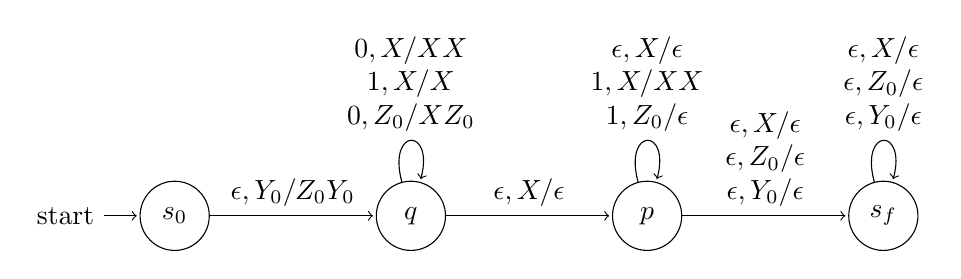
\begin{tikzpicture}[shorten >=1pt,node distance=3cm,on grid,auto,bend angle=45] 
   \node[state,initial] (s0)   {$s_0$}; 
   \node[state] (q) [right=of s0] {$q$}; 
   \node[state] (p) [right=of q] {$p$}; 
   \node[state](sf) [right=of p] {$s_f$};
    \path[->] (s0) edge  node {$\epsilon, \Y/Z_{0}\Y$} (q);
    \path[->] (q) edge  node  {$\epsilon, X/\epsilon$} (p);
    \path[->] (q) edge [loop above] node [align=center]  {$0,X/XX$\\ $1, X/X$ \\$0,Z_{0}/XZ_{0}$} (q);
    \path[->] (p) edge  node [align=center] {$\epsilon , X / \epsilon$ \\ $\epsilon , Z_{0} / \epsilon$ \\ $\epsilon, \Y / \epsilon$} (sf);
    \path[->] (p) edge [loop above] node [align=center] {$\epsilon, X/\epsilon$\\ $1, X/XX$ \\$ 1,Z_{0}/\epsilon$} (p) ;
    \path[->] (sf) edge [loop above] node [align=center] {$\epsilon, X/\epsilon$ \\ $\epsilon, Z_{0}/\epsilon$ \\ $\epsilon, \Y/\epsilon$} (sf);
\end{tikzpicture}\\[0.5cm]
\footnotesize Fig. PDA $P_{1}$ with acceptance by empty stack
\end{center}
\newpage
%}}}
% 3.2 Find a PDA P2 such that $L(P_{2}) = N(P)$
%{{{
\subsection{Find a PDA P2 such that $L(P_{2}) = N(P)$}
\htab Find a PDA $P_{2}$ such that $L(P_{2}) = N(P)$; i.e., $P_{2}$ accepts by final state what $P$ accepts by empty stack. \pg
\htab To establish an equivalent PDA $P_{2}$ with acceptance by final state, we utilize an additional state $s_{0}$ to introduce the initial bottom of statck $Z_{0}$ in the original PDA $P$, and another new state $s_{f}$ as final state of new PDA $P_{2}$.\\
\htab The $P_{2}$ we construct is $(\{s_{0}, s_{f}, p, q\}, \{ 0, 1\}, \{\Y, Z_{0}, X\}, \delta, \Y, s_{0}, \{s_{f}\})$, transition functions are as follows,
    \begin{align}
        \delta(q, 0, Z_{0}) &= \{ (q, XZ_{0})\} \\
        \delta(q, 0, X) &= \{ (q, XX)\} \\
        \delta(q, 1, X) &= \{ (q, X) \} \\
        \delta(q, \epsilon, X) &= \{ (p, \epsilon)\} \\
        \delta(p, \epsilon, X) &= \{ (p, \epsilon)\} \\
        \delta(p, 1, X) &= \{ (p, XX)\} \\
        \delta(p, 1, Z_{0}) &= \{ (p, \epsilon)\} \\
        \delta(s_{0}, \epsilon, \Y) &= \{ (q, Z_{0}\Y)\} \label{PDA2:new1} \\
        \delta(q, \epsilon, \Y) &= \{ (s_{f}, \epsilon)\}\label{PDA2:new2} \\
        \delta(p, \epsilon, \Y) &= \{ (s_{f}, \epsilon)\} \label{PDA2:new3} 
    \end{align}
\htab Then is the graphical representation of new PDA $P_{2}$,\\
\begin{center}
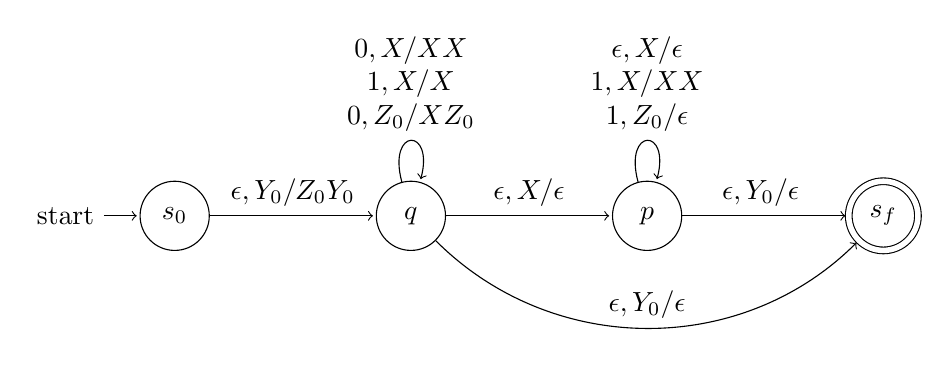
\begin{tikzpicture}[shorten >=1pt,accepting/.style={double distance=2pt},node distance=3cm,on grid,auto,bend angle=45] 
   \node[state,initial] (s0)   {$s_0$}; 
   \node[state] (q) [right=of s0] {$q$}; 
   \node[state] (p) [right=of q] {$p$}; 
   \node[state,accepting](sf) [right=of p] {$s_f$};
    \path[->] (s0) edge  node {$\epsilon, \Y/Z_{0}\Y$} (q);
    \path[->] (q) edge  node  {$\epsilon, X/\epsilon$} (p);
    \path[->] (q) edge [loop above] node [align=center]  {$0,X/XX$\\ $1, X/X$ \\$0,Z_{0}/XZ_{0}$} (q);
    \path[->] (q) edge [bend right] node [align=center] {$\epsilon, \Y / \epsilon$} (sf);
    \path[->] (p) edge  node [align=center] {$\epsilon , \Y / \epsilon$ } (sf);
    \path[->] (p) edge [loop above] node [align=center] {$\epsilon, X/\epsilon$\\ $1, X/XX$ \\$ 1,Z_{0}/\epsilon$} (p) ;
\end{tikzpicture}\\[0.5cm]
\footnotesize Fig. PDA $P_{2}$ with acceptance by final state
\end{center}
\newpage
%}}}

% Exercise 4
\section{From Grammar to PDA}
\htab Convert the grammar
    $$ S \rightarrow aAA $$
    $$ A \rightarrow aS \ba bS \ba a $$
\htab to a PDA that accepts the same language by empty stack, and show an accepting sequence of IDs for input string $aabaaa$.
% 4.1 Conversion to PDA 
%{{{
\subsection{Conversion to PDA $\ps$}
\htab Based on the given grammer, construct a PDA with acceptance by empty stack 
$\ps (Q, \Sigma, T, q_{s}, \delta, I)$ whose formal definition is 
\begin{itemize} 
    \item State sets $Q = \{q\}$  
    \item Alphabet of Input String $\Sigma = \{a, b\}$  
    \item Stack Symbols $T = \{S, A, a, b\}$  
    \item Start State $q_{s} = q$  
    \item Initial symbol in the stack $I = S$  
    \item Transition functions $\delta$ are defined as follows, (here write $\delta (q, \epsilon, A)$ separately for better reference)
\end{itemize}
    \begin{align}
        \delta (q, \epsilon, S) &= \{(q, aAA)\} \label{ps1} \\
        \delta (q, \epsilon, A) &= \{(q, aS), (q, bS), (q, a)\} \label{ps2}\\
        \delta (q, a, a) &= \{(q, \epsilon)\} \label{ps5}\\
        \delta (q, b, b) &= \{(q, \epsilon)\} \label{ps6} 
    \end{align}
%}}}
% 4.2 Show sequence of IDs
%{{{
\subsection{Show sequence of IDs for $aabaaa$}
\htab The sequence of IDs is presented to show acceptance of string $aabaaa$ by $\ps$, the number over the derivation mark is index of the transition equation based on which that step of derivation is made,
\begin{align}
    \pdaid{aabaaa}{S} 
    & \idDerive{\eqref{ps1}} \pdaid{aabaaa}{aAA} &&\mbox{by \eqref{ps1}} \\
    & \idDerive{\eqref{ps5}} \pdaid{abaaa}{AA} &&\mbox{pop $a$ by \eqref{ps5}}\\
    & \idDerive{\eqref{ps4}} \pdaid{abaaa}{aA} &&\mbox{pop $A$, push $a$ by \eqref{ps2}}\\
    & \idDerive{\eqref{ps5}} \pdaid{baaa}{A} &&\mbox{pop $a$ by \eqref{ps5}} \\
    & \idDerive{\eqref{ps3}} \pdaid{baaa}{bS} &&\mbox{pop $A$, push $bS$ by\eqref{ps2}}\\
    & \idDerive{\eqref{ps6}} \pdaid{aaa}{S} &&\mbox{pop $b$ by \eqref{ps6}} \\
    & \idDerive{\eqref{ps1}} \pdaid{aaa}{aAA} &&\mbox{pop $S$, push $aAA$ by \eqref{ps1}} \\
    & \idDerive{\eqref{ps5}} \pdaid{aa}{AA} &&\mbox{pop $a$ by \eqref{ps5}} \\
    & \idDerive{\eqref{ps4}} \pdaid{aa}{aA} &&\mbox{pop $A$, push $a$ by \eqref{ps2}}\\
    & \idDerive{\eqref{ps5}} \pdaid{a}{A} &&\mbox{pop $a$ by \eqref{ps5}} \\
    & \idDerive{\eqref{ps4}} \pdaid{a}{a} &&\mbox{pop $A$, push $a$ by \eqref{ps2}}\\
    & \idDerive{\eqref{ps5}} \pdaid{\epsilon}{\epsilon} &&\mbox{pop $a$ by \eqref{ps5}} \\
    & \Rightarrow accepted &&\mbox{acceptance by empty stack}
\end{align}
\newpage
%}}}

% Exercise 5 Pumping Lemma TBD
%{{{
\section{Use of CFL Pumping Lemma}
\subsection{Show language $ \{ a^{i} b^{j} c^{k} \ba i \times j = k \} $ not to be context-free}
\htab Use the CFL pumping lemma to show the following language not to be context-free: 
    $$ \{ a^{i} b^{j} c^{k} \ba i \times j = k \} $$ 
\htab First, we assume that the language 
    \begin{equation} \label{pp:assumption}
        L = \{ a^{i} b^{j} c^{k} \ba i \times j = k \}\ is\ context\ free\ language. 
    \end{equation}
\htab Consider the $ z = a^{2n} b^{n} c^{ 2n^{2} } $ for arbitrary $n$. \\
\htab Decompose the word, we have $ z = uvwxy $ 
    \begin{equation} z = uvwxy \end{equation}
\htab Such decomposition is valid because the length of $z$,
    \begin{equation} 2n+n+2n^{2} \geq n \end{equation}
\htab By pumping lemma, the following condition is satisfied since $L$ is context-free language, 
    \begin{align}
        |vwx| \leq n  \label{pp:lessthann} \\
        |vx| > 0  \label{pp:nonzero} \\
        \forall r \geq 0, uv^{r}wx^{r}y \in L \label{pp:pump}
    \end{align}
\htab Since the length of $vwx$ is restricted to be at most $n$, all possibibilities for assignment of $v$ and $x$ are easier to be detected. And also we should show that in each case, after pumping $v$ and $x$, the word $z$ is no longer in the language $L$.
\begin{itemize} \renewcommand{\labelitemii}{$\diamond$}
    \item{$vwx$ is all $a$s, in this case, both $v$ and $x$ must be all $a$s. If we dumplicate the $v$ and $x$, the number of $a$s in resulting word will increase, while the number of $b$s and $c$s remain unchanged. The resulting word does not satisfy $i \times j = k $ any more and thus not in language $L$.}
    \item{$vwx$ is all $b$s, in this case, both $v$ and $x$ must be all $b$s. If we dumplicate the $v$ and $x$, the number of $b$s in resulting word will increase, while the number of $a$s and $c$s remain unchanged. The resulting word does not satisfy $i \times j = k $ any more and thus not in language $L$.}
    \item{$vwx$ is all $c$s, in this case, both $v$ and $x$ must be all $c$s. If we dumplicate the $v$ and $x$, the number of $c$s in resulting word will increase, while the number of $a$s and $b$s remain unchanged. The resulting word does not satisfy $i \times j = k $ any more and thus not in language $L$.}
    \item{$vwx$ consists of $a$s and $b$s, in this case, $v$ consist of $a$s or possibly $a$s with some $b$s, and $x$ consists of $bs$ or possibly $bs$ with some $a$s. If we dumplicate the $v$ and $x$, the number of $a$ and $b$ in resulting word will increase, while the number of $c$s remain unchanged. The resulting word does not satisfy $i \times j = k $ any more and thus not in language $L$.}
    \item{$vwx$ is combination of $b$ and $c$, specific scenarios are showns in the following. }
     \begin{itemize}
         \item{$v$ consists of only $bs$, $x$ consists of only $cs$. Since all cases we talked about here has one or more $b$, suppose the number of $b$ in $v$ is $p\geq 1$. Now we want to duplicate the $v$ and $x$. To keep the resulting word satisfy the property $i \times j = k $, the number of $c$ in $x$ must be $2n\times p$, which is impossible because we have restricted the length of $vwx$ to be smaller than or equal to $n$. (here $|vwx| > |x| = 2np > n$)}
         \item{$v$ consists of only $bs$, $x$ consists of $bs$ and $cs$. Obviously, duplicating the $x$ will violate the form of $a^{i} b^{j} c^{k}$, hence the result would never in language $L$. }
        \item{$v$ consists of $bs$ and $cs$, $x$ is all $cs$. Obviously, duplicating the $v$ will violate the form of $a^{i} b^{j} c^{k}$, hence the result would never in language $L$.}
     \end{itemize}
\end{itemize}
\htab As we can see from the analysis above, in all cases, \eqref{pp:pump}
is contradicted after pumping or duplicating of $v$ and $x$ for $r$ times.
Therefore, we should negate our assumption \eqref{pp:assumption} at the beginning.\\
\htab Hence, we sucessfully prove that 
\begin{equation} \{ a^{i} b^{j} c^{k} \ba i \times j = k \} \ is \ not \ context\ free\ language \end{equation}
\newpage
%}}}

% Exercise 6 Closure Property
%{{{
\section{Closures Properties of CFLs}
\subsection{Show $max(\cdot)$ has no closure property for CFL}
\htab Show that the CFLs are \textit{not} closed under the following operation:
\begin{center}
    $max(L)$ = \{w $|$ w is in $L$ and for no $x$ other than $\epsilon$ is $wx$ in $L$\}
\end{center}
\htab \textbf{Proof}: \\
\htab First of all, we assume that context-free language is closed under the $max(\cdot)$ operator. 
Hence, we have 
\begin{align}
    \forall \text{context-free language } L, max(L) \text{ is also context-free language.}
    \label{6:assumeClosure}
\end{align}
\htab And then pick out a language $\LL = \{0^{i}1^{j}2^{k} \ba i \geq k\ or\ j \geq k\}$, which is a context-free
because we can easily construct a context-free grammar $E$ to genereate this language, 
\begin{align}
    E &\rightarrow AB \ba D \\
    A &\rightarrow A0 \ba \epsilon \\
    B &\rightarrow 1B \ba 1B2 \ba \epsilon \\
    D &\rightarrow 0D \ba F \\
    F &\rightarrow 0F2 \ba G \\
    G &\rightarrow G1 \ba \epsilon 
    \end{align}
\htab Note that, we guarantee that $j \geq k$ if $E$ is instantiated to $AB$, 
and we secure that $i \geq k$ if $E$ is instantiated to $D$. \\
\htab After verifying that the $\LL$ we pick up is context-free language, we start to
show the language $max(\LL)$, which is processed by operator $max(\cdot)$,
is not context-free language. \\
\htab Based on the given definition of operator $max(\cdot)$, we can derive 
the form of $max(\LL)$ as follows,
\begin{align}
    max(\LL) = \{ 0^{i}1^{j}2^{k} \ba k = max(i,j) \} \label{6:maxl}
    \end{align}
\htab Now prove the $max(\LL)$ is not contex-free language by pumping lemma. \\
\htab We assume that the language $max(\LL)$ in \eqref{6:maxl} is context-free language.\\
\htab Consider the string $s = 0^{Q} 1^{Q} 2 ^{Q}$, which is obviously in $max(\LL)$. 
($Q$ is an arbitrary constant.)
Since the language $max(\LL)$ is a context-free language by our assumption, we can
decompose the string $s$ into five part, that is,
\begin{align}
     s = uvwxy ,\ | uvwxy | &\geq Q
    \end{align}
\htab Such that,
\begin{align}
    | vwx | &\leq Q\\
    | vx | &> 0 \\
    \forall z \geq 0,\ & uv^{z}wx^{z}y \in max(\LL) \label{6:ppl}
    \end{align}
\htab Now we make analysis for all possible assignment of $vwx$, since the length of $vwx$ is limited, the string $vwx$ cannot access all three different characters at the same time.
\begin{itemize}
    \item{if $vwx$ consists of only $0s$, pump $v$ and $x$ will make resulting $s'=uv^{z}wx^{z}y$ remain in $max(\LL)$, but if we duplicate the $v$ and $x$, in which way $k \neq max(i,j) $ since the $i$ has increased but $k$ kept unchanged, the resulting $s'$ will be not in $max(\LL)$. Hence, \eqref{6:ppl} does not hold in this case.} 
    \item{if $vwx$ consists of only $1s$, similar to the all-0 case, pump $v$ and $x$ will make resulting $s'$ remain in $max(\LL)$, but if we duplicate the $v$ and $x$, in which way $k \neq max(i,j) $ since the $j$ has increased but $k$ kept unchanged, the resulting $s'$ will be not in $max(\LL)$. Hence, \eqref{6:ppl} does not hold in this case.} \\
\vfill 
\hrule
{
\footnotesize The condition provided by pumping lemma in \eqref{6:ppl} says no matter pumping or duplicting $v$ and $z$ for any times, the resulting string must remain in the context-free language.
}
    \item{if $vwx$ consists of only $2s$, pumping or duplication of $v$ and $x$ will make the resulting $s'$ not in $max(\LL)$ in that the $k$ has a different value while the $i$ and $j$ remained unvaried.  Hence, \eqref{6:ppl} does not hold in this case.}
\item{if $vwx$ consists of $0s$ and $1s$, \eqref{6:ppl} does not hold in all possible scenarios of this case as follows:}
    \begin{itemize} \renewcommand{\labelitemii}{$\diamond$}
        \item{if $v$ consists of both $0s$ and $1s$, and $x$ only consists of $1s$, the duplicated string will not be in the form $0^{i}1^{j}2^{k}$.}
        \item{if $v$ consists of only $0s$, and $x$ consists of both $0s$ and $1s$, the duplicated string will not be in the form $0^{i}1^{j}2^{k}$.}
        \item{if $v$ consists of only $0s$ and $x$ consists of only $1s$, any pumping or duplication of $v$ and $x$ will make the resulting $s'$ not in $max(\LL)$ in that both $i$ and $j$ changed but $k$ has no move.}
    \end{itemize}   
    \item{if $vwx$ consists of $1s$ and $2s$, \eqref{6:ppl} does not hold in all possible scenarios of this case as follows:}
    \begin{itemize} \renewcommand{\labelitemii}{$\diamond$}
        \item{if $v$ consists of both $1s$ and $2s$, and $x$ only consists of $2s$, the duplicated string will not be in the form $0^{i}1^{j}2^{k}$.}
        \item{if $v$ consists of only $1s$, and $x$ consists of both $1s$ and $2s$, the duplicated string will not be in the form $0^{i}1^{j}2^{k}$.}
        \item{if $v$ consists of only $1s$ and $x$ consists of only $2s$, duplication of $v$ and $x$ may keep the resulting $s'$ in $max(\LL)$ if $|v| = |x|$, but pumping $v$ and $x$ inevitably break the $k = max(i,j)$ since the $max(i,j)$ is $i$, which has no variation.}
    \end{itemize}   
\end{itemize}
\htab In summary, for all possible assignment of $vwx$, the \eqref{6:ppl} does not hold for $max(\LL)$. That is to say, we find a conflict for the assumption made before that the $max(\LL)$ is context-free language. Hence, we ought to negate the assumption. Therefore, we have 
\begin{center}
    the language $max(\LL)$ is not context-free language.
    \end{center}
\htab Thus, we find a example $\LL$ to illustrate that if $L$ is context-free language, its maximized language $max(L)$ is not necessary to be context-free language. Formally,
\begin{center}
    $\exists$ context-free language $L$, $max(L)$ is \textit{not} context-free language.\\[0.2cm]
    \end{center}
\htab which contradicts to what we have derived in \eqref{6:assumeClosure} 
    by assuming the closure property of $max(\cdot)$ in the very beginning. \pg
\htab As the consequence of this second contradiction, we negate the assumption in the very beginning and obtain
\begin{align}
    \text{CFLs are \textit{not} closed under the operator } max(\cdot) 
    \end{align}
\newpage
%}}}
\end{document}
    
